% chapters/introduction.tex
%
% Copyright 2022 Alexander Lyttle.
%
% This work may be distributed and/or modified under the conditions of the
% LaTeX Project Public License (LPPL) version 1.3 or later.
%
% The latest version of this license is in
% https://www.latex-project.org/lppl.txt and version 1.3 or later is part of
% all distributions of LaTeX version 2005/12/01 or later.
%
%
\chapter[Inferring Stellar Parameters with Asteroseismology]{Inferring Stellar Parameters with Asteroseismology}

\textit{In this chapter, I introduce the current state of modelling stars with asteroseismology and the types of stars being studied in this thesis. I start with a brief history of understanding the stars spanning the last century. In Section \ref{sec:seismo}, I introduce asteroseismology of stars which oscillate like the Sun. Then, I provide examples of asteroseismology being used to model large samples of dwarf and subgiant stars in Section \ref{sec:many-stars}. Finally, I introduce the concept of modelling stars the `Bayesian way' with some examples of current methods and their limitations.}

% Since the late 19th century, astronomers have been trying to understand the physical structure and evolution of the Sun and other stars. They wanted to determine whether other stars were like the Sun and whether they changed with time. Answers to these questions could tell us where we came from and what the future holds for the solar system. While little was known of this at the time, astronomers started by gathering data in an effort to map the night sky. The invention of the spectrograph by \citet{Draper1874} allowed researchers to systematically classify stars by their brightness in different wavelengths of light \citep{Maury.Pickering1897}. This was an pivotal early step towards the large-scale stellar surveys we are used to today.

% \citet{Hertzsprung1909} made early estimates of absolute magnitude from the widths of the spectral lines

\section{Understanding the Stars}\label{sec:stars}

Early efforts to understand the stars began by finding relations between their spectral classification and magnitude in different photometric bands. On what was later called a Hertzsprung-Russell (HR) diagram \citep[e.g.][]{Russell1914}, astronomers plot the absolute magnitude (or luminosity, \(L\)) of a star against its spectral class (or effective temperature, \(\teff\)). They found that stars were not uniformly distributed on the HR diagram, but were instead grouped in distinct sequences. For example, the narrow diagonal band where most stars were found was called the \emph{main sequence}. Astronomers wondered why stars adhered to these sequences and to what extent they evolved with time.

Initial insight into stellar evolution came about when astronomers studied open clusters on the HR diagram \citep{Trumpler1930}. These are groups of stars found at a similar distance and close together on the sky. Assuming clusters formed at the same time with similar chemical abundances, the only expected difference between stars is their mass and multiplicity. Using stars of known mass (e.g. from orbital solutions to binary systems) and luminosity distributions, astronomers could trace lines of similar mass and composition from younger to older clusters \citep[e.g.][]{Sandage1957}. Coupled with early arguments from stellar physics \citep[e.g.][]{Chandrasekhar1939}, scientists formed stellar evolutionary tracks --- the path a star takes on the HR diagram during its evolution. Deriving the stellar radius (\(R\)) from the relation \(L \propto R^2 \teff^4\), they inferred that stars started life on the dimmer edge of the main sequence and became brighter and larger throughout most of their lifetime. At some point, stars would leave the main sequence, rapidly cool, expand, and then ascend a region of the HR diagram known as the \emph{red giant branch}.

%  \citet{Kuiper1938} found an empirical mass-luminosity relation.

% Explaining structure in the HR diagram involved studying open clusters of stars. Astronomers expected these groups of stars, found at a similar parallax, to have formed at a similar time with similar chemical abundances. They presumed the remaining variation was for stars of different mass. Therefore, ordering open clusters on an HR diagram showed the evolution of stars of different mass. Furthermore, early measurements of stellar mass came from orbital solutions to visual and spectroscopic binary star systems.

% Observations of stars in clusters, assumed to have similar ages and chemical abundances, showed how stars of different mass evolved across the HR diagram with time.

% The luminosity and effective temperature could be estimated from the magnitude and colour of the stars. From luminosity and temperature, we could derive the radius of stars. Early stellar mass estimates came from visual and spectroscopic binaries. Spectroscopy provides abundances of chemical species ionised in the stellar atmosphere. However, except for the Sun, stellar age and helium abundance has no model-independence. The latter ionisations at temperatures and densities higher than the surface of stars like the Sun.

The chemical composition, energy sources and evolutionary physics of stars were still uncertain. Spectroscopy revealed relative abundances of elements excited in stellar atmospheres, but it was difficult to determine their absolute abundances. \citet{Payne1925} proposed that stars comprised mostly hydrogen and helium, later reinforced by estimates of helium content in the Sun \citep[e.g.][]{Schwarzschild1946}. The idea was radical at the time because it did not match the abundance of elements found on Earth. Meanwhile, advancements in nuclear science spawned the theory of stellar nucleosynthesis \citep{Hoyle1946}. Stars produce elements heavier than hydrogen and helium through nuclear fusion reactions. This discovery explained the production of many elements in the universe, tying the formation and evolution of stars to planetary formation and the conditions for life in the universe.

In the second half of the 20th century, astronomers advanced the theory of stellar evolution. With this came computational methods for simulating stars \citep[e.g.][]{Kippenhahn.Weigert.ea1967}. Astronomers could start to compare observations of stars and clusters with numerical solutions to stellar structure equations. We call this process \emph{modelling stars}. Early models of the Sun benefited from independent geological age estimates and neutrino-production rates from observing cosmic rays. With these constraints, and the Sun as a calibrator, researchers could start to refine their models and test them on other stars. For example, \citet{Iben1967} computed stellar models for main sequence stars with similar masses to the Sun using observations of the clusters M67 and NGC 188.

On a similar timescale, a new field emerged which gave astronomers a model-independent way of studying the inside of stars. Identifying regular perturbations of the surface of the Sun, researchers realised that they pertained to high-order, stochastically-driven spherical harmonic oscillations. Measuring these oscillation modes, they could study the Sun similarly to how seismologists study the Earth. Astronomers studying multiple non-radial stellar oscillations distinguished this new field, called \emph{asteroseismology}, from the well-known study of radially pulsating stars \citep[e.g. Cepheid variables;][]{Leavitt1908}. In Section \ref{sec:seismo} we briefly elaborate on the history and theory of asteroseismology for stars like the Sun.

% Approximations for the equation of state by \citet{Eggleton.Faulkner.ea1973}.

Today, astronomers have a huge abundance of data with which to determine stellar parameters and test theories of stellar evolution. In Section \ref{sec:many-stars}, we give some recent examples of Sun-like asteroseismic populations and their context in the wider HR diagram. With big datasets and complex, multi-parameter models, there has been a recent shift towards Bayesian statistical methods to model these stars. Therefore, we introduce the concept of modelling stars `the Bayesian way' in Section \ref{sec:modelling-stars}. There, we introduce some tools used to model these stars and then highlight some common assumptions made.

% Large-scale surveys have lead to asteroseismology on a large scale. Combined with photometry, spectroscopy and astrometry (parallax, position and motion), asteroseismology has bePowerful tool in Section \ref{sec:many-stars}.

% Modelling stars became a way to test theories of stellar evolution and estimate the ages of stars. In recent years, the Bayesian framework...  

% We briefly introduce modelling stars the Bayesian way in Section \ref{sec:modelling-stars}.

% On a similar timescale, the field of helioseismology emerged. Starting by observing oscillations on the surface of the Sun. When applied to other stars, asteroseismology. This gave highly precise measurements of the oscillation modes. Solar-like oscillators oscillate like the Sun. These provided an independent way to test stellar models and determine masses and radii from the scaling relations.

\section[Solar-Like Oscillators]{Asteroseismology of Solar-Like Oscillators}\label{sec:seismo}

% In this section, we provide a brief history and theory of asteroseismology to provide a foundation from which to understand this thesis. However, we recommend the recent review by \citet{Aerts2021} or the lecture notes by \citet{Christensen-Dalsgaard2014} for a more detailed understanding of the field.

\subsection{A Brief History of Asteroseismology}

Several decades ago, 5-minute oscillations in the radial velocity of the solar surface were observed by \citet{Leighton.Noyes.ea1962}, leading to the inference of acoustic waves trapped beneath the solar photosphere \citep{Ulrich1970}. A further decade of study culminated in the measurement of regular patterns of oscillation modes in the Sun; for example, from measurements of radial velocity \citep{Claverie.Isaak.ea1979} and total irradiance \citep{Woodard.Hudson1983a}. Initially thought to be short-lived irregularities on the surface, these modes were found to be compatible with stochastically excited standing waves penetrating deep into the Sun. Later, \citet{Deubner.Gough1984} introduced the word \emph{helioseismology} to describe the study of the solar interior using observations of these modes. Helioseismology was soon responsible for breakthrough solar research, from measuring differential rotation \citep{Deubner.Ulrich.ea1979} to solving the mismatch between predicted and measured solar neutrino production \citep{Bahcall.Ulrich1988}.

Astronomers initially debated the mechanism driving the modes of standing pressure waves (or p modes) in the Sun. \citet{Goldreich.Keeley1977} suggested what became the prevailing theory, that the p modes were stochastically excited by near-surface convection. Therefore, astronomers expected solar-like oscillations to be present in other stars with a convective envelope like the Sun. Shortly thereafter, \citet{Christensen-Dalsgaard1984} was among those to introduce the term \emph{asteroseismology} --- the study of the internal structure of stars with many observable oscillation modes. Subsequently, solar-like oscillations were discovered in a few bright stars. Among the first were Procyon and \(\alpha\) Cen A \citep{Gelly.Grec.ea1986}, with individual modes later resolved by \citet{Martic.Schmitt.ea1999} and \citet{Bouchy.Carrier2001} respectively.

Instrumental and atmospheric noise limited the progress of asteroseismology with ground-based equipment to studies of small number of bright dwarf stars. Asteroseismology of solar-like oscillators requires high-cadence (\(\sim \SIrange{1}{10}{\minute}\)) brightness observations over long baselines (\(\sim \SI{1}{\year}\)) with parts-per-million precision \citep[e.g.][]{Schofield.Chaplin.ea2019}. 
% For example, noise of \(\lesssim \SI{100}{ppm\per\hour}\) for \(I\)-band magnitudes \(\lesssim 10\) \citep{Schofield.Chaplin.ea2019}. 
The first dedicated space-based missions which met these requirements arrived in the late 2000s, accelerating progress in the field. Initially, the \emph{CoRoT} mission \citep{Baglin.Auvergne.ea2006} detected solar-like oscillations in thousands of red giant stars \citep{DeRidder.Barban.ea2009,Mosser.Belkacem.ea2010}. Then, the \emph{Kepler} mission \citep{Borucki.Koch.ea2010} yielded oscillations in thousands more red giants \citep{Pinsonneault.Elsworth.ea2014} and hundreds of main sequence stars similar to the Sun \citep{Serenelli.Johnson.ea2017}. Most recently, \emph{TESS} \citep{Ricker.Winn.ea2015} added thousands more dwarf and giant stars to the roster of solar-like oscillators \citep{Hon.Huber.ea2021,SilvaAguirre.Stello.ea2020,Hatt.Nielsen.ea2023}. For a more detailed review of modern asteroseismology, see \citet{Aerts2021}. 

\subsection{A Brief Theory of Solar-Like Oscillations}\label{sec:seismo-theory}

\begin{figure}[tb]
    \centering
    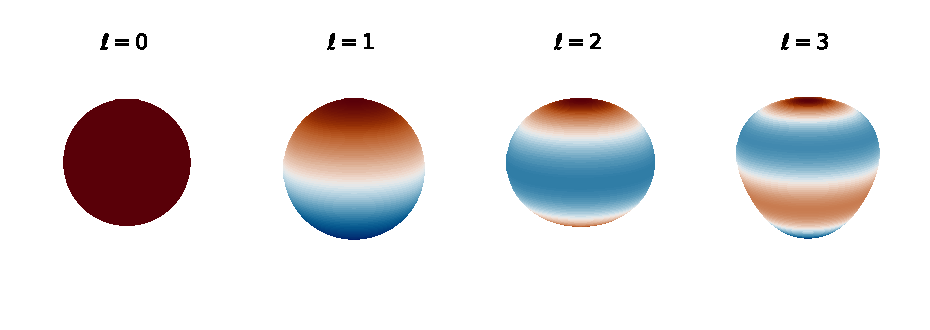
\includegraphics[trim={0 0.4in 0 0},clip]{figures/spherical_harmonics.pdf}
    \caption[Surface spherical harmonic oscillation modes for a few angular degrees ($l$) with azimuthal order \(m=0\).]{Surface spherical harmonic oscillation modes for a few angular degrees ($l$) with azimuthal order \(m=0\). The colour-map represents radial displacement at the surface, with \emph{red} and \emph{blue} corresponding to displacement inward and outward respectively. The coloured regions pulsate in and out, and the white regions represent stationary nodes on the surface.}
    \label{fig:spherical-harmonics}
\end{figure}

We can approximate oscillations on the surface of a star by spherical harmonic functions with angular degree \(l\) and azimuthal order \(m\),
%
\begin{equation}
    Y_l^m (\theta, \varphi) \propto P_l^m (\cos\theta) \, \ee^{im\varphi},
\end{equation} 
%
where \(\theta\) is the polar angle, \(\varphi\) is the azimuthal angle, and \(P_l^m\) is the associated Legendre polynomial. The angular degree is the number of nodes on the surface of the star. We show a representation of the surface spherical harmonics for the first four angular degrees in Figure \ref{fig:spherical-harmonics}. For each \(l\), there exists \(2l+1\) solutions with different azimuthal order (\(m\)) corresponding to the different orientations of the nodes over the spherical surface. Additionally, the oscillation modes have unique frequency solutions for different radial orders (\(n\)) proportional to the number of nodes radially throughout the star.

\begin{figure}[tb]
    \centering
    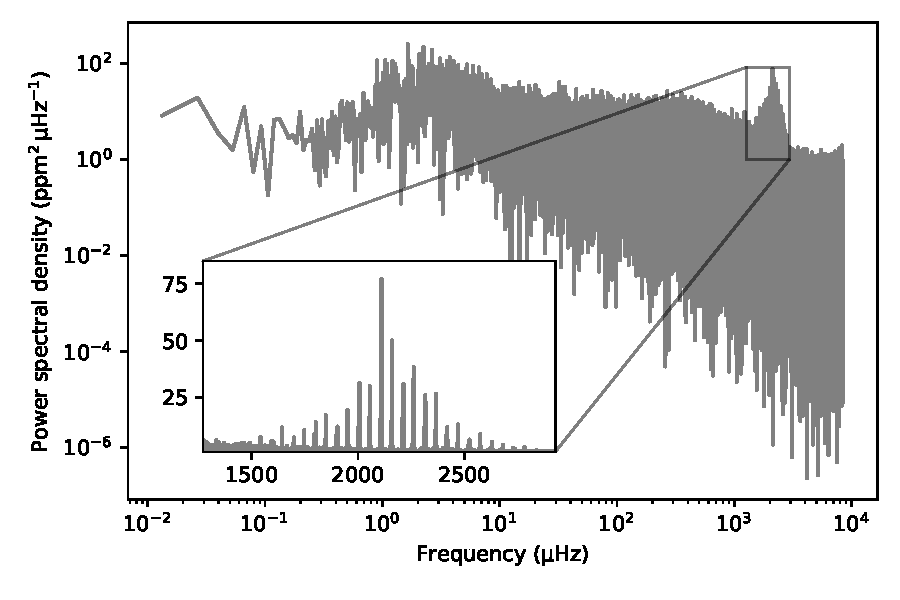
\includegraphics{figures/seismo-psd.pdf}
    \caption[The power spectral density of 16 Cyg A.]{The power spectral density of 16 Cyg A. The inset plot highlights the Gaussian-like power excess in the larger plot.}
    \label{fig:seismo-psd}
\end{figure}

In solar-like oscillators, p modes are stochastically excited by near-surface convection. Typically, the timescale of this process drives high-order modes in main sequence stars (\(n \sim 20\)). We can identify these modes in a frequency-power spectrum derived from photometric or radial velocity time series observations. For instance, both stars in the 16 Cygni planet hosting system are solar-like oscillators with similar properties to the Sun \citep{Metcalfe.Chaplin.ea2012,Davies.Chaplin.ea2015,Metcalfe.Creevey.ea2014}. Using 16 Cyg A as an example, we downloaded the power spectrum determined by the \emph{Kepler} Asteroseismic Science Operations Centre (KASOC) using \emph{Kepler} observations\footnote{\url{https://kasoc.phys.au.dk}}. Shown in Figure \ref{fig:seismo-psd}, the power spectrum of 16 Cyg A has a distinct power excess around \SI{2000}{\micro\hertz}. 

The power excess has a Gaussian-like shape around frequencies compatible with the near-surface convective timescale responsible for mode excitation. We call the centre of this Gaussian the \emph{frequency at maximum power} (\(\numax\)). Dependent on near-surface conditions, \citet{Brown.Gilliland.ea1991} suggested \(\numax\) scales with the acoustic cut-off frequency --- the highest frequency at which acoustic waves can reflect near the stellar surface. Subsequently, \citet{Kjeldsen.Bedding1995} found that \(\numax \propto g\teff^{\,-1/2}\) where \(g\) and \(\teff\) are the near-surface gravitational field strength and effective temperature. Hence, \(\numax\) for a solar-like oscillator decreases as it evolves, from \(\sim \SI{1000}{\micro\hertz}\) on the main sequence to \(\sim \SI{10}{\micro\hertz}\) near the tip of the red giant branch.

Looking closely at the power excess in Figure \ref{fig:seismo-psd}, we can see a comb of approximately equally spaced peaks. Each peak corresponds to an oscillation mode, with their collective central frequencies and separations providing information about the internal stellar structure. Naturally, higher frequency modes correspond to higher radial order, \(n\). However, the angular degree and azimuthal order are harder to identify. We saw in Figure \ref{fig:spherical-harmonics} how modes of higher \(l\) have more anti-nodes on the surface. Therefore, the overall effect of the oscillations cancel out when measuring irradiance integrated over the stellar surface. Consequentially, observed mode amplitude decreases with \(l\), leaving only \(l \lesssim 3\) detectable. 
% Not Section 2.1 of JCD Lecture Notes (2014) derives this
Therefore, we can assume the tallest peaks are \(l=0,1\), and the smaller peaks are \(l=2,3\), all modulated by the wider Gaussian-like envelope.

Modes with different \(m\) cannot be distinguished for a spherically symmetric, non-rotating star. In the case of a rotating or distorted (asymmetric) star, the observed mode frequencies will split for different \(m\) via the Doppler effect. Measuring this splitting can constrain the rotation rate of the star \citep[e.g.][]{Davies.Chaplin.ea2015,Garcia.Ceillier.ea2014,Deheuvels.Garcia.ea2012}. Such studies have lead to breakthrough research on the rotational evolution of stars \citep[e.g.][]{Angus.Aigrain.ea2015,Hall.Davies.ea2021,vanSaders.Ceillier.ea2016}. However, we will hereafter consider only the case of a slowly rotating, spherically symmetric star.

For an acoustic wave in a one-dimensional homogeneous medium, we would expect each mode of oscillation to be an integer multiple of the fundamental mode. While the case for a star is more complicated, we can also approximate the frequencies for different modes as a multiple of a characteristic frequency. \citet{Tassoul1980} found that the modes could be approximated by assuming the asymptotic limit, where \(l/n \rightarrow 0\). This lead to the following expression for the frequency of a mode for a given \(n\) and \(l\) \citep[cf.][]{Gough1986},
%
\begin{equation}
    \nu_{nl} \simeq \left(n + \frac{l}{2} + \varepsilon\right) \nu_0 + O(\nu_{nl}^{-1}), \label{eq:asy}
\end{equation}
%
where \(\varepsilon\) is some constant offset and \(O(\nu_{nl}^{-1})\) represents higher order terms. The characteristic frequency (\(\nu_0\)) is the inverse of the acoustic diameter (sound crossing time),
%
\begin{equation}
    \nu_0 = \left(2 \int_{0}^{R} \frac{\dd r}{c(r)}\right)^{-1},
\end{equation}
%
where \(c(r)\) is the sound speed as a function of radius (\(r\)), and \(R\) is the radius of the star. Similarly to other variable stars, \citet{Ulrich1986} found that this characteristic frequency relates to mean stellar density by \(\nu_0 \propto \overline{\rho}^{\,1/2}\). While \(\nu_0\) is not directly detectable in solar-like oscillators, we can approximate it by taking the difference between consecutive modes of the same angular degree, \(\Delta\nu_{nl} = \nu_{nl} - \nu_{n-1\,l}\). Thus, estimates of a global (or average) \emph{large frequency separation}, \(\Delta\nu\), can also provide information about the density of a star. This leads to independent constraint on stellar mass and radius (e.g. from scaling relations to the Sun).

\begin{figure}[tb]
    \centering
    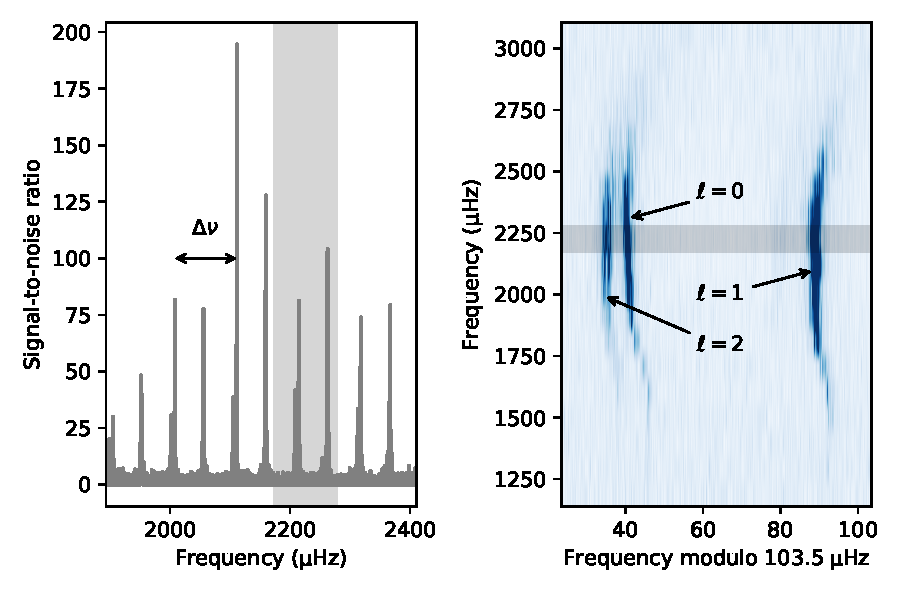
\includegraphics{figures/seismo-echelle.pdf}
    \caption[Signal-to-noise ratio as a function of frequency and echelle diagram for 16 Cyg A.]{\emph{Left:} A section of the spectral signal-to-noise ratio (SNR) against frequency for 16 Cyg A. The large frequency spacing (\(\Delta\nu\)) between two radial modes is annotated with a double-headed arrow. The shaded region corresponds to a single row (also highlighted) in the echelle plot. \emph{Right:} The echelle plot shows the spectral SNR such that a darker colour represents a higher SNR. Each row spans \SI{103.5}{\micro\hertz} and is stacked in order of frequency. The apparent ridges are labelled according to the angular degree (\(l\)) of the modes they represent.}
    \label{fig:seismo-echelle}
\end{figure}

The asymptotic expression helps us identify modes in a star. If the first term of Equation \ref{eq:asy} was exact, we would expect odd and even modes to be grouped together and separated by \(\dnu/2\). To show this, we revisit the power spectrum of 16 Cyg A and estimate a signal-to-noise ratio (SNR) by dividing out a moving median in log-frequency steps of \SI{0.005}{\dex}. We can see the regular pattern predicted by Equation \ref{eq:asy} in the left panel of Figure \ref{fig:seismo-echelle}. Every other mode is approximately separated by \(\dnu\). To see this effect over the wider spectrum, we created an \emph{echelle} plot in the right panel. Folding the spectrum by an estimate of \(\dnu\) reveals a sequence of ridges corresponding to modes of different angular degree. Odd and even angular degree are grouped together, although do not lie on top of each other. The small difference between modes of different \(l\) is described by the higher order terms neglected from Equation \ref{eq:asy}. A faint ridge corresponding to \(l=3\) modes is also visible next to the \(l=1\) ridge. However, 16 Cyg A represents one of the highest SNR dwarf stars observed by \emph{Kepler}, and the \(l=3\) ridge is otherwise not usually visible. 

% Once we have identified a solar-like oscillator, what information is there to gain from asteroseismology? We have discussed how parameters \(\numax\) and \(\dnu\) scale with global stellar properties. Scaling these parameters with respect to the Sun, we can obtain relations for the radius and mass of the star,
% %
% \begin{align}
%     \left(\frac{R}{\si{\solarradius}}\right) &\simeq \left(\frac{\numax}{\numax_{,\odot}}\right) \left(\frac{\dnu}{\dnu_\odot}\right)^{-2} \left(\frac{\teff}{\teff_{,\odot}}\right)^{1/2},\\
%     \left(\frac{M}{\si{\soNonlarmass}}\right) &\simeq \left(\frac{\numax}{\numax_{,\odot}}\right)^3 \left(\frac{\dnu}{\dnu_\odot}\right)^{-4} \left(\frac{\teff}{\teff_{,\odot}}\right)^{3/2}.
% \end{align}
% %
% Using these relations directly can provide quick-look, independent mass and radius estimates \citep[e.g.][]{Pinsonneault.Elsworth.ea2018}.

% We can also use individual modes and compare with models. Worth noting the surface term here.

Repeating this kind of analysis on a large-scale can provide a wealth of observables from which to model stars. In the next section, we give some examples where asteroseismology was used to model many solar-like oscillators.

\section[Modelling Stars with Asteroseismology]{Modelling Many Stars with Asteroseismology}\label{sec:many-stars}

Recent space-based missions like \emph{Kepler} and \emph{TESS} enable asteroseismology with many stars. These missions were primarily designed to detect exoplanets using the transit method. However, their instrumental requirements were also well-suited to asteroseismology. This allowed astronomers to study regions of the HR diagram in more detail, from main sequence dwarf stars to red giants. We draw particular attention to \emph{Kepler}, the first of the two missions. \emph{Kepler}'s primary mission observed a single \(\sim\SI{100}{deg\squared}\) patch of sky for around 4 years \citep{Borucki.Koch.ea2010}, cut short by a mechanical failure which spawned the secondary \emph{K2} mission \citep{Howell.Sobeck.ea2014}. \emph{Kepler} took photometric measurements in long (\SI{30}{\minute}) and short (\SI{60}{\second}) cadences, with the Nyquist frequency of the latter high enough to detect main sequence oscillators. During its primary mission, large asteroseismic datasets were gathered. The long baseline of 4 years allowed for high frequency precision not since seen by \emph{K2} or \emph{TESS}.

% In this section, we introduce the sample of stars being studied in this thesis relative to the broader astronomical picture.

Of the asteroseismic targets found by \emph{Kepler}, we focus on dwarf and subgiant solar-like oscillators. These are stars with a similar mass to the Sun on the main sequence or shortly after the turn-off before ascending the red giant branch. From an asteroseismic perspective, the power spectra of dwarf stars are relatively simple. As solar-like oscillators approach the red giant branch, their modes begin to couple with buoyancy-driven modes in the core \citep{Bedding.Mosser.ea2011,Mosser.Barban.ea2011}. This leads to irregular patterns which can be used to separate evolutionary state and study properties of the core \citep[e.g.][]{Mosser.Vrard.ea2015}. On the other hand, the relative simplicity of main sequence oscillators make them a suitable place to start our study. Furthermore, the work in this thesis anticipates the upcoming \emph{PLATO} mission which aims to observe \(\sim 10^4\) dwarf and subgiant oscillators \citep{Rauer.Aerts.ea2016}.

% Modelling many stars with asteroseismology is complemented by other recent large-scale stellar surveys. High-precision astrometry from the \emph{Gaia} mission \citep{GaiaCollaboration.Prusti.ea2016} has provided improved distances and orbital solutions. The APOGEE large-scale spectroscopic survey \citep{Majewski.Schiavon.ea2017} has also yielded precise chemical abundances. These surveys have enabled studies of the assembly history of our galaxy. For example, \citet{Helmi.Babusiaux.ea2018} discovered a merger between the Milky Way and Gaia-Enceladus by analysing the motions and abundances from \emph{Gaia} and APOGEE. Asteroseismology has accompanied this work by helping determine the ages of stars tied to the merger \citep{Chaplin.Serenelli.ea2020,Montalban.Mackereth.ea2021}.

Modelling many stars with asteroseismology is complemented by other recent large-scale stellar surveys. High-precision astrometry from the space-based \emph{Gaia} mission provides precise distances and orbital solutions for over a billion sources \citep{GaiaCollaboration.Prusti.ea2016}. Additionally, the APOGEE large-scale spectroscopic survey provides precise chemical abundances for over half a million targets to date \citep{Majewski.Schiavon.ea2017,Jonsson.Holtzman.ea2020}. When combined, these surveys have enabled studies of the assembly history of our galaxy \citep[e.g.][]{Helmi.Babusiaux.ea2018} which have since been strengthened by asteroseismology \citep{Chaplin.Serenelli.ea2020,Montalban.Mackereth.ea2021}.

\begin{figure}
    \centering
    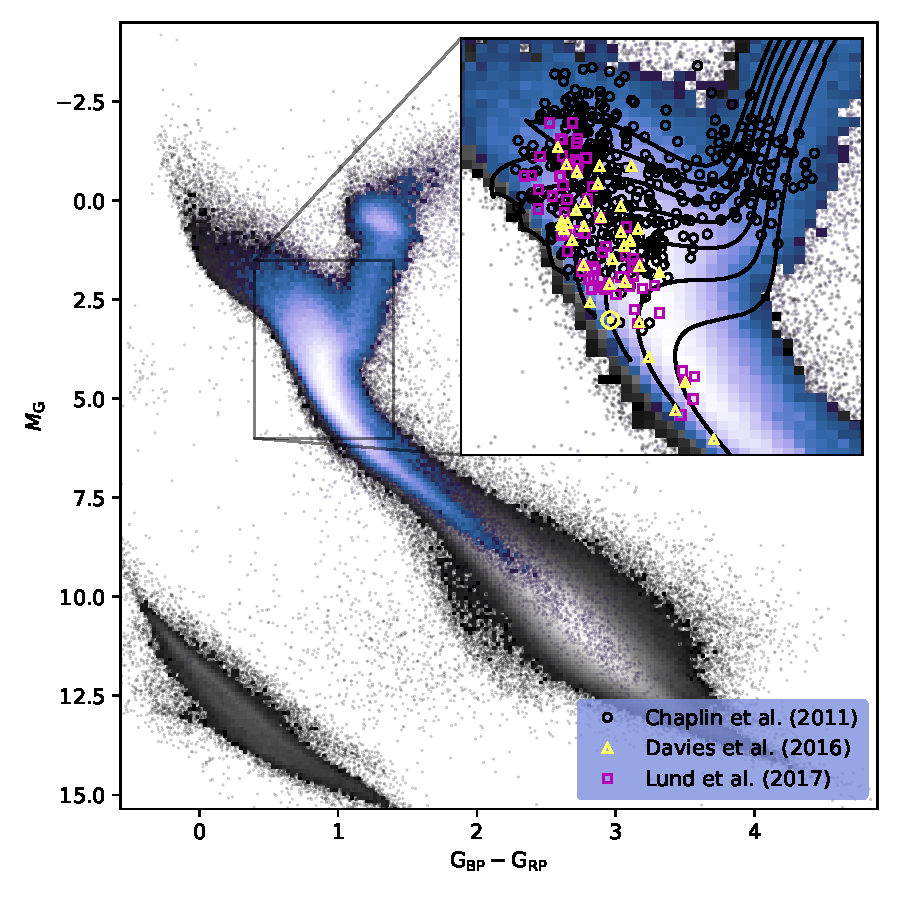
\includegraphics{figures/hr-diagram.pdf}
    \caption[Colour-magnitude diagram highlighting the region occupied by dwarf and subgiant solar-like oscillators.]{Colour-magnitude diagram highlighting the region occupied by solar-like oscillators. 
    % The data are \emph{Gaia} G, G\textsubscript{BP}, and G\textsubscript{RP} band magnitudes respectively. The absolute magnitude (\(M_\mathrm{G}\)) is calculated from \emph{Gaia} parallaxes neglecting extinction. 
    \emph{Main plot:} The background 2D histogram (greyscale) shows the density of \emph{Gaia} DR3 targets with parallax \(>\SI{5}{\milli\aarcsec}\) (distance \(\lesssim\SI{200}{\parsec}\)). The foreground 2D histogram (blue-purple) shows the density of all \emph{Kepler} targets in \emph{Gaia} DR3. Scattered points are shown where the density is less than 10 points per bin.
    \emph{Inset plot:} Stellar evolutionary tracks with solar metallicity are given by the black lines for \SIrange{0.8}{1.4}{\solarmass} in steps of \SI{0.1}{\solarmass}. The circles in the inset axes correspond to \emph{Kepler} solar-like oscillators with references given in the legend. The Sun is given by the `\(\odot\)' symbol.}
    \label{fig:hr-diagram}
\end{figure}

In Figure \ref{fig:hr-diagram}, we show a colour-magnitude diagram made using magnitudes and parallaxes from \emph{Gaia} Data Release 3 \citep[DR3;][]{GaiaCollaboration.Vallenari.ea2022}. For this illustrative plot, we have neglected the effect of extinction from dust in the interstellar medium. The background distribution shows solar-neighbourhood \emph{Gaia} sources with a parallax greater than \SI{5}{\milli\aarcsec} for context. Over-plot is the distribution of \emph{Kepler} objects cross-matched with \emph{Gaia} DR3\footnote{The cross-matched dataset was obtained from \url{https://gaia-kepler.fun}}. The densest region lies in the low- to intermediate-mass main sequence (\SIrange{0.8}{1.2}{\solarmass}) but we can also see a clear red giant branch and red clump in the upper-right of the distribution. The inset plot draws attention to the region occupied by dwarf and subgiant solar-like oscillators, where we give some examples.

\citet{Chaplin.Kjeldsen.ea2011} identified the first large catalogue of \(\sim 500\) dwarf and subgiant solar-like oscillators (black circles in Figure \ref{fig:hr-diagram}) by measuring \(\dnu\) and \(\numax\) in \emph{Kepler} data. Later, \citet{Chaplin.Basu.ea2014} determined ages, masses and radii for these stars using \(\dnu\) and \(\numax\) complemented by photometry and ground-based spectroscopy where available. The subsequent arrival of APOGEE spectroscopy allowed \citet{Serenelli.Johnson.ea2017} to revisit this sample with a more consistent set of \(\teff\) and metallicity. By comparing observations to models of stellar evolution, they found radii, masses and ages with uncertainties of around 3, 5 and 20 per cent respectively.

For a subset of these stars, the SNR was high enough to identify many individual modes. \citet{Appourchaux.Chaplin.ea2012} were among the first to publish individual mode frequencies (\(\nu_{nl}\)) for around 60 of these stars. This sample was later modelled by \citet{Metcalfe.Creevey.ea2014} who found observing individual modes doubled precision of radii, masses and ages over using \(\dnu\) and \(\numax\) alone. Around the same time, the number of confirmed exoplanets was increasing rapidly \citep{Burke.Bryson.ea2014}. This motivated a more detailed study of 35 exoplanet host stars by \citet{SilvaAguirre.Davies.ea2015} with modes identified by \citet{Davies.SilvaAguirre.ea2016}. We can see these as yellow triangles in Figure \ref{fig:hr-diagram}. The remaining best targets, referred to as the LEGACY sample, were modelled by \citet{SilvaAguirre.Lund.ea2017} using modes identified by \citet{Lund.SilvaAguirre.ea2017}. We show these as magenta squares in Figure \ref{fig:hr-diagram}.

% These targets are still being studied extensively today helium glitch \citet{Mazumdar.Monteiro.ea2014,Verma.Raodeo.ea2019}.

% While we have introduced the data used in modelling stars with asteroseismology, we have not explained how parameters like radius, mass and age are determined. In the next section, we introduce how these stars are modelled using Bayesian methodology. 

% However, there have been many sources of systematic uncertainty. Many assumptions were made in the modelling of this sample of stars. It is a perfect test case for new modelling methods. Then the plan is to apply these to future missions like Plato and Nancy Grace Roman.

\section{Modelling Stars the Bayesian Way}\label{sec:modelling-stars}

% The phrase `modelling stars' can be confusing. We often use it to describe the process of numerically simulating the physics of a star. Some examples of such simulations are one-dimensional stellar evolution codes (e.g. MESA) and three-dimensional hydrodynamical simulations \todo{e.g. other}. However, we also use the word `model' in probabilistic inference to refer to the process of generating predictions with some set of model parameters given some observed data \citep[e.g.][]{Hogg.Bovy.ea2010}. In this thesis, we prefer the phrase `modelling stars' to mean the entire process of inferring stellar parameters using a generative model. To model a given star, we may need to compute many stellar simulations, but the overall model compares these simulations to data in a probabilistic way. To avoid confusion where possible, we refer to numerical models of stars as either stellar simulations or evolutionary models.

% In some cases, stellar parameters can be estimated from observables using direct or empirical relationships. For example, mass-luminosity relation, or asteroseismic scaling relations.

% With the advent of high-precision asteroseismology for many stars, astronomers have a plethora of observables to constrain physical models of stellar evolution. 

% A la carte modelling involves producing and optimising dedicated stellar models for a given star. Many parameters can be optimised this way, but it is slow.

% Grid-based modelling involves producing a large grid of stellar models and computing the likelihood across the grid. Some examples. Assumptions must be made on approximations of stellar physics such as helium and MLT. Also overshoot, diffusion, rotation, solar abundances and opacity tables.

Modelling stars `the Bayesian way' involves estimating the probability distributions of stellar parameters (\(\vect{\theta}\)) given observed parameters (\(\vect{y}\)). For example, the parameters of interest might be the age, mass and initial fractional heavy-element abundance of the star (\(\vect{\theta} = t_\star, M, Z\)) and we might observe the effective temperature, luminosity, and large frequency spacing (\(\vect{y} = \teff, L, \Delta\nu\)). We can do this starting with Bayes' theorem for the \emph{posterior} probability density,
%
\begin{equation}
    p(\vect{\theta} \mid \vect{y}) = \frac{p(\vect{y} \mid \vect{\theta})\,p(\vect{\theta})}{p(\vect{y})},\label{eq:bayes-theorem}
\end{equation}
%
where \(p(\vect{y} \mid \vect{\theta})\) is the \emph{likelihood}, \(p(\vect{\theta})\) is the \emph{prior}, and \(p(\vect{y})\) is the \emph{evidence}. We should choose a prior to represent our expectation for \(\vect{\theta}\). The prior dominates if the observations are bad (i.e. have a small likelihood) and we return our current `belief' (or expectation). However, if the observations are good enough, the likelihood has more influence on the posterior and our belief is updated. As a result, we can use the Bayesian methodology to systematically update our beliefs. This provides a statistical scheme from which to build our stellar models.

Let us consider a stellar model with three parameters, \(\vect{\theta} = t_\star, M, Z\). For instance, we might want the age of a star to help date a galactic merger, or its mass to characterise an exoplanetary system. To get the probability distribution of age given our observations, we must \emph{marginalise} over the joint posterior with respect to all other parameters. The marginal posterior probability distribution for \(t_\star\) is,
%
\begin{equation}
    p(t_\star \mid \vect{y}) = \int\limits_0^\infty \int\limits_0^1 p(\vect{\theta} \mid \vect{y}) \, \dd M \dd Z,
\end{equation}
%
where the bounds of the integral are chosen across all space for \(M\) and \(Z\). In other words, the marginal distribution involves integrating over the uncertainty in all other model parameters.

The marginal posterior distribution depends on our choice of function which maps \(\vect{\theta}\) to predict observable parameters, \(\tilde{\vect{y}} = f(\vect{\theta})\). The likelihood then compares the predictions (\(\tilde{\vect{y}}\)) with observations (\(\vect{y}\)). When modelling stars, there is no analytical form to \(f\). Instead, we use numerical simulations which take in \(\vect{\theta}\) and approximate \(\vect{y}\). For example, Modules for Experiments in Stellar Astrophysics \citep[MESA; originally developed by][]{Paxton.Bildsten.ea2011} is a one-dimensional stellar evolution code. Assuming spherical symmetry, MESA simulates the structure and evolution of a star along a one-dimensional radial slice. The code numerically solves a series of differential equations which govern the interior dynamics of the star \citep[see, e.g.][for an introduction to stellar structure and evolution]{Kippenhahn.Weigert.ea2013}. Often starting with a cloud of gas, MESA evolves the system over dynamical time steps recording physical properties at mesh points inside the star.

We can also predict oscillation mode frequencies (\(\nu_{nl}\)) with simulations. For example, the GYRE code developed by \citet{Townsend.Teitler2013} uses the output of MESA to compute oscillation modes for a given \(n\) and \(l\). While the physics of p mode propagation in the star is relatively well-known, our understanding of the atmospheric boundary conditions are not. As such, there is a known discrepancy between the simulated and observed p modes. The nature of this can lead to a systematic bias when modelled \(\dnu\) and \(\nu_{nl}\). Corrections for this effect exist \citep[e.g.][]{Ball.Gizon2014} but are still not fully understood.

The complexity of stellar models means that the marginalised posterior distributions are not analytically derivable. One solution is to estimate the posterior with numerical methods like Markov Chain Monte Carlo (MCMC). Typically, this involves exploring parameter space with multiple calls to \(f\) for different values of \(\vect{\theta}\). In the case of MCMC-based algorithms like Hamiltonian Monte Carlo (HMC) and the No U-Turn Sampler (NUTS), the gradient of \(f\) is also required. There are several open-source \textsc{Python} packages widely used to implement these algorithms, for instance \texttt{pymc} \citep{Salvatier.Wiecki.ea2016} and \texttt{numpyro} \citep{Phan.Pradhan.ea2019}.

There are some existing methods for determining stellar parameters using this Bayesian approach. As an early example, \citet{Bazot.Bourguignon.ea2008} used the MCMC algorithm to sample model parameters with on-the-fly stellar model calculation. While their method could be tailored to individual stars, it was very computationally expensive. Each proposed set of \(\vect{\theta}\) spawns a stellar simulation which evolves to a given age. Steps prior to this age may be discarded, and the simulation can take minutes to hours for each set of \(\vect{\theta}\). This was not a viable solution for modelling the large populations of stars being observed with high-precision today.

A more efficient solution is to sample a discrete grid of models \citep{Gruberbauer.Guenther.ea2012,Gruberbauer.Guenther.ea2013}. For example, a recent tool which does this is the BAyesian STellar algorithm (BASTA) developed by \citet{AguirreBorsen-Koch.Rorsted.ea2022}. The authors pre-compute and interpolate a grid of simulated stars corresponding to a set of relevant input parameters. They weight the grid points according to the prior and then compute the marginalised posterior for each model parameter. We could extend this by interpolating a grid of stellar models to approximate \(f\) itself. This is done in the Asteroseismic Inference on a Massive Scale (AIMS) pipeline by \citet{Lund.Reese2018,Rendle.Buldgen.ea2019}. However, interpolation methods can be slow. They scale poorly with dimensionality and number of points on the grid. A small subset of the grid can be used to mitigate this issue, but we want a solution which can be extended to model many stars at once.

Asteroseismology has allowed us to model stars more precisely than ever before. This has exposed systematic uncertainties in common assumptions used when computing these models \citep[e.g.][]{Tayar.Claytor.ea2022}. For instance, fractional helium abundance (\(Y\)) cannot be determined spectroscopically in cool stars. Instead, we often assume it follows a linear enrichment law \citep{Chiosi.Matteucci1982,Ribas.Jordi.ea2000,Casagrande.Flynn.ea2007}. Such a law assumes that helium is enriched in the interstellar medium linearly with metallicity. However, \citet{Lebreton.Goupil.ea2014} found that varying \(Y\) by \(\pm\,0.03\) can have \(\gtrsim \mp\,20\) per cent effect on stellar age. Therefore, assuming \(Y\) instead of incorporating it in our model leads to underestimating our uncertainty on stellar age and other correlated parameters. In Chapters \ref{chap:glitch} and \ref{chap:glitch-gp}, we will explore one way to improve inference of \(Y\) using an asteroseismic signature of helium ionisation. In the meantime, we explore a better statistical treatment of our prior on such poorly characterised parameters.

% Another assumption is the value of the mixing-length theory parameter (\(\mlt\)). This parametrises a common approximation of convective mixing used in stellar models \citep{Gough1977}. Many of the aforementioned methods assume a value of \(\mlt\) calibrated to the Sun. However, 3D hydrodynamical models have shown different values of \(\mlt\) do a better job of approximating convection for different stars \citep{Magic.Weiss.ea2015}.

% To properly model stars the Bayesian way, we need to accommodate \(Y\) and \(\mlt\) in our models. Unfortunately, the effect of these parameters on observables is degenerate. Observables are not precise enough to differentiate between the two on a star-by-star level. 

Finally, it is important that our prior represents not only our belief for individual stars, but also the population. There are many cases where we would expect stellar parameters to be correlated between stars. Not accounting for such correlations cause us to overestimate uncertainty on individual stellar parameters. For example, we believe that \(Y\) belongs to a distribution governed by chemical enrichment of the interstellar medium. Stars formed in a similar place and time should share similar chemical abundances. We can incorporate prior beliefs like this using a hierarchical Bayesian model (HBM). In the next chapter, we introduce the concept of an HBM. We explore a simple HBM in the context of astronomy and show how it can improve our estimates of stellar parameters. Following that, we present a hierarchical model on a population of dwarf and subgiant stars observed by \emph{Kepler} in Chapter \ref{chap:hmd}.

% While such a method improves upon and tackles bias in our choice of \(Y\) and \(\mlt\), there is more helium abundance information to be gained from asteroseismology. Finally, in Chapter \ref{chap:glitch}, we explore signatures of helium abundance in the oscillation modes of stars. We present a new method for characterising these glitches.
